%chktex-file 1 chktex-file 2 chktex-file 3
%chktex-file 8 chktex-file 9 chktex-file 10
%chktex-file 13 %chktex-file 17 %chktex-file 23
%chktex-file 45 %chktex-file 25 %chktex-file 35
%chktex-file 40

\documentclass[oneside,12pt,a4paper]{report}

\usepackage{template}

\begin{document}

    \begin{center}
        \fontsize{17.28}{17.28}
            \textbf{Equações Diferenciais Ordinárias}

            \textbf{Segunda Lista de Exercícios}
    \end{center}

%%%%%%%%%%%%%%%%%%%%%%%%%%%%%%%%%%%%%%%%%%%%%%%%%%%%%%%%%
% QUESTÕES
%%%%%%%%%%%%%%%%%%%%%%%%%%%%%%%%%%%%%%%%%%%%%%%%%%%%%%%%%


    \exercicio[Zill, Seção 2.1, Exercício 15 (a)] Esboce as curvas de isóclinas $f(x,y)=c$ para a equação diferencial
    \[\frac{dy}{dx}=x+y\quad-5\leq c\leq 5,~c\in\mathbb{Z}\] 
    usando os valores indicados de $c$. Construa um campo direcional sobre uma malha desenhando cuidadosamente elementos lineares com a inclinação apropriada nos pontos escolhidos em cada curva de isóclina. Use este campo direcional para esboçar uma curva solução aproximada para o PVI consistindo na ED e nas condições iniciais $y(0)=1$.

    \exercicio[Zill, Seção 2.1, Exercícios 21, 23, 28] Encontre os pontos críticos e o retrato de fase de cada equação diferencial de primeira ordem dada. Classifique cada ponto crítico como assintoticamente estável, instável ou semiestável. Esboce à mão curvas integrais típicas nas regiões do plano $xy$ determinadas pelos gráficos das soluções de equilíbrio.
    \begin{itensquestao}[3]
        \item $\dfrac{dy}{dx}=y^2-3y$
        \item $\dfrac{dy}{dx}=(y-2)^4$
        \item $\dfrac{dy}{dx}=\dfrac{ye^y-9y}{e^y}$
    \end{itensquestao}

    \exercicio[Zill Seção 2.2, Exercícios 2, 6, 11, 13, 17, 21] Resolva, por separação de variáveis, as equações diferenciais dadas.
    \begin{itensquestao}[2]
        \item $e^xy\dfrac{dy}{dx}=e^{-y}+e^{-2x-y}$
        \item $\dfrac{dy}{dx} = \left(\dfrac{2y+3}{4x+5}\right)^2$
        \item $\mathrm{cossec}(y)dx+\sec^2(x)dy=0$
        \item $(e^y+1)^2e^{-y}dx+(e^x+1)^3e^{-x}dy=0$
        \item $\dfrac{dP}{dt}=P-P^2$
        \item $\dfrac{dy}{dx}=x\sqrt{1-y^2}$
    \end{itensquestao}

    \exercicio[Zill Seção 2.2, Exercício 38] Mostre que uma solução implícita de \[2x\sin^2(y)dx-(x^2+10)\cos(y)dy=0\] é dada por $\ln(x^2+10)+\mathrm{cossec}(y)=c$. Ache as soluções constantes, se houver, que foram perdidas na solução da equação diferencial.

    \exercicio[Zill Seção 2.2, Exercícios 49, 50] Nos itens a) e b), use uma técnica de integração ou uma substituição para encontrar uma solução explícita do problema de valor inicial.
    \begin{itensquestao}[2]
        \item $\dfrac{dy}{dx}=\dfrac{e^{\sqrt{x}}}{y},\quad y(1)=4$
        \item $\dfrac{dy}{dx}=\dfrac{x\arctan(x)}{y},\quad y(0)=3$
    \end{itensquestao}

    \exercicio[Zill Seção 2.3, Exercícios 3, 12, 14, 21] Ache a solução geral da equação diferencial dada. Dê o maior intervalo $I$ sobre o qual a solução geral está definida. Determine se há termos transientes na solução geral.
    \begin{itensquestao}[2]
        \item $\dfrac{dy}{dx}+y=e^{3x}$
        \item $(1+x)\dfrac{dy}{dx}-xy=x+x^2$
        \item $xy'+(1+x)y=e^{-x}\sin(2x)$
        \item $\dfrac{dr}{d\theta}+r\sec{\theta}=\cos{\theta}$
    \end{itensquestao}

    \exercicio[Zill Seção 2.3, Exercício 37] Resolva o problema de valor inicial dado. Use um software gráfico para representar a função contínua $y(x)$.
        \[\dfrac{dy}{dx}+2y=f(x),~\text{onde}~f(x)=
        \begin{cases}
            1,\quad0\leq x\leq 3\\
            0,\quad x>3
        \end{cases},~y(0)=0\]

    \exercicio[Zill Seção 2.3, Exercício 42] Considere o problema de valor inicial $y'+e^xy=f(x),~y(0)=1$. Expresse a solução do PVI para $x>0$ como uma integral não elementar quando $f(x)=1$. Qual é a solução quando $f(x)=0$? E quando $f(x)=e^x$?

    \exercicio[Zill Seção 2.4, Exercícios 11, 15, 17, 18] Determine se a equação diferencial dada é exata. Se for, resolva-a.
    \begin{itensquestao}[1]
        \item $(y\ln(y)-e^{-xy})dx+\left(\dfrac{1}{y}+x\ln(y)\right)dy=0$
        \item $\left(x^2y^3-\dfrac{1}{1+9x^2}\right)\dfrac{dx}{dy}+x^3y^2=0$
        \item $(\tan(x)-\sin(x)\sin(y))dx+\cos(x)\cos(y)dy=0$
        \item $(2y\sin(x)\cos(x)-y+2y^2e^{xy^2})dx=(x-\sin^2(x)-4xye^{xy^2})dy$
    \end{itensquestao}

    \exercicio[Zill Seção 2.4, Exercícios 24, 26] Resolva os problemas de valor inicial dados.
    \begin{itensquestao}[1]
        \item $\left(\dfrac{3y^2-t^2}{y^5}\right)\dfrac{dy}{dt}+\dfrac{t}{2y^4}=0,\quad y(1)=1$
        \item $\left(\dfrac{1}{1+y^2}+\cos(x)-2xy\right)\dfrac{dy}{dx}=y(y+\sin(x)),\quad y(0)=1$
    \end{itensquestao}

    \exercicio[Zill Seção 2.4, Exercícios 37, 38] Resolva o problema de valor inicial dado encontrando um fator integrante apropriado.
    \begin{itensquestao}[1]
        \item $xdx+(x^2y+4y)dy=0,~y(4)=0$
        \item $(x^2+y^2-5)dx=(y+xy)dy,~y(0)=1$
    \end{itensquestao}

    \exercicio[Zill Seção 2.5, Exercícios 6, 8, 10, 13] Cada uma das EDs é homogênea. Resolva a equação diferencial ou problema de valor inicial dados por meio de uma substituição apropriada.
    \begin{itensquestao}[1]
        \item $(y^2+yx)dx+x^2dy=0$
        \item $\dfrac{dy}{dx}=\dfrac{x+3y}{3x+y}$
        \item $x\dfrac{dy}{dx}=y+\sqrt{x^2-y^2},\quad x>0$
        \item $(x+ye^{y/x})dx-xe^{y/x}dy=0, \quad y(1)=0$
    \end{itensquestao}

    \exercicio[Zill Seção 2.5, Exercícios 16, 17, 20, 21] Cada uma das EDs é uma equação de Bernoulli. Resolva a equação diferencial ou problema de valor inicial por meio de uma substituição apropriada.
    \begin{itensquestao}[1]
        \item $\dfrac{dy}{dx}-y=e^xy^2$
        \item $\dfrac{dy}{dx}=y(xy^3-1)$
        \item $3(1+t^2)\dfrac{dy}{dx}=2ty(y^3-1)$
        \item $x^2\dfrac{dy}{dx}-2xy=3y^4,\quad y(1)=\dfrac{1}{2}$
    \end{itensquestao}

    \exercicio[Zill Seção 2.5, Exercícios 24, 25, 27] Cada uma das EDs é da forma $y'=f(Ax+By+C)$. Resolva a equação diferencial ou problema de valor inicial por meio de uma substituição apropriada.
    \begin{itensquestao}[1]
        \item $\dfrac{dy}{dx}=\dfrac{1-x-y}{x+y}$
        \item $\dfrac{dy}{dx}=\tan^2(x+y)$
        \item $\dfrac{dy}{dx}=2+\sqrt{y-2x+3}$
        \item $\dfrac{dy}{dx}=\cos(x+y),\quad y(0)=\dfrac{\pi}{4}$
    \end{itensquestao}

%%%%%%%%%%%%%%%%%%%%%%%%%%%%%%%%%%%%%%%%%%%%%%%%%%%%%%%%%
% RESOLUÇÕES
%%%%%%%%%%%%%%%%%%%%%%%%%%%%%%%%%%%%%%%%%%%%%%%%%%%%%%%%%

\chapter*{Resolução dos Exercícios}
        
    \begin{resolucao}
        \definecolor{quivercolor}{HTML}{73B0FF}
        \definecolor{isocolor}{HTML}{C9C9C9}

        Para resolver o exercício, primeiramente, devemos determinar as equações das curvas de isóclina que usaremos. Assim, como $x+y=c$, reescrevemos $y=c-x,~c\in\mathbb{Z},~-5\leq c\leq5$. Traçando essas curvas, temos

        \begin{figure}[H]
            \centering
            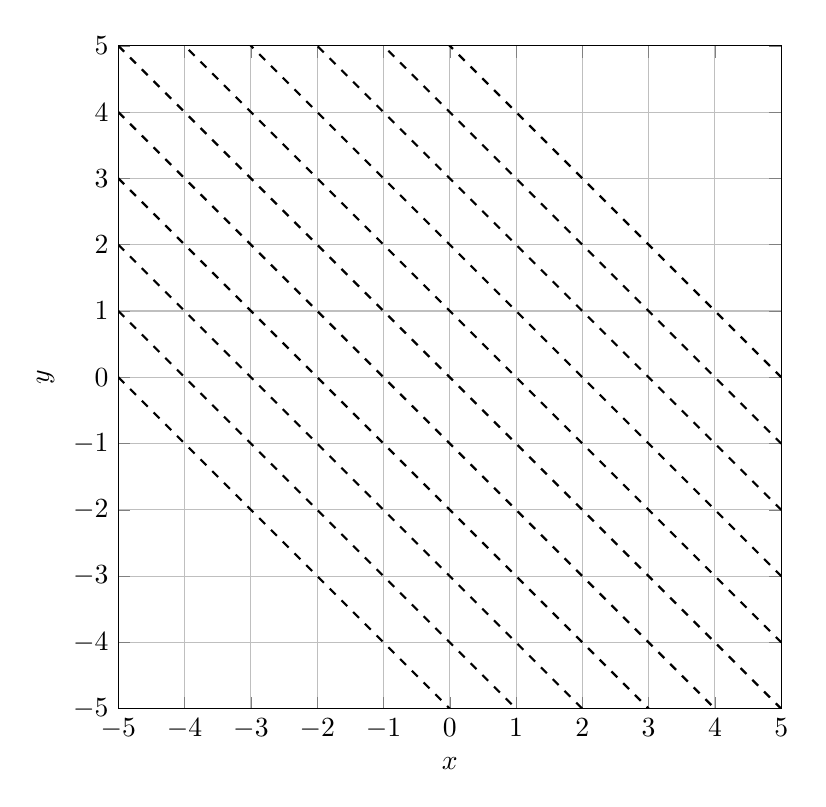
\begin{tikzpicture}
            \begin{axis}[
                width=10cm,
                height=10cm,
                view={0}{90},
                xmin=-5, xmax=5,
                ymin=-5, ymax=5,
                axis equal image, % Garante a proporção correta
                grid=major,
                xtick={-5,-4,...,5},
                ytick={-5,-4,...,5},
                xlabel={$x$},
                ylabel={$y$},
                % Corta qualquer coisa desenhada fora da área do gráfico (ex: a extrapolação)
                restrict y to domain=-10:10, 
                clip=true
            ]

            % 2. Isóclinas (c = -5 a 5)
            \pgfplotsinvokeforeach{-5,-4,...,5}{
                \addplot [
                    domain=-5:5, 
                    samples=2, 
                    dashed, 
                    color=black, 
                    thick
                ] {#1 - x};
            }

            \end{axis}
            \end{tikzpicture}
        \end{figure}

        Em seguida, devemos traçar os elementos lineares com inclinação $\dfrac{dy}{dx}=c$ sobre cada isóclina $x+y=c$, compondo assim o campo direcional

        \begin{figure}[H]
            \centering
            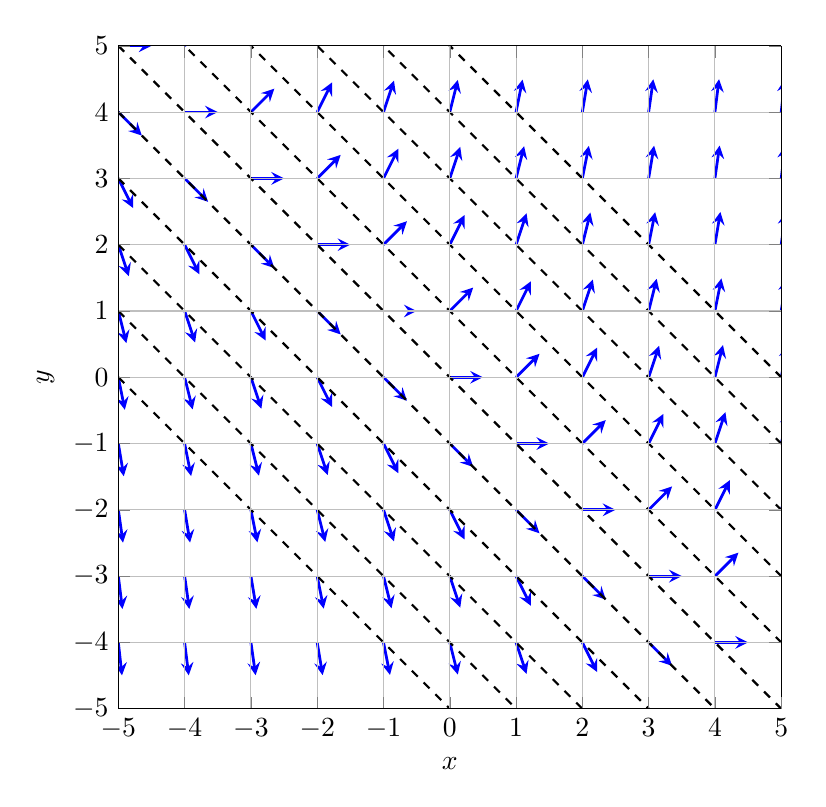
\begin{tikzpicture}
            \begin{axis}[
                width=10cm,
                height=10cm,
                view={0}{90},
                xmin=-5, xmax=5,
                ymin=-5, ymax=5,
                axis equal image, % Garante a proporção correta
                grid=major,
                xtick={-5,-4,...,5},
                ytick={-5,-4,...,5},
                xlabel={$x$},
                ylabel={$y$},
                % Corta qualquer coisa desenhada fora da área do gráfico (ex: a extrapolação)
                restrict y to domain=-10:10, 
                clip=true
            ]

            % 1. Campo Direcional (Quiver)
            % Obs: O pgfplots vai desenhar o campo em toda a malha. 
            % Se o vetor sair da área, o 'clip=true' corta automaticamente.
            \addplot3 [
                quiver={
                    u={1 / sqrt(1 + (x+y)^2)},
                    v={(x+y) / sqrt(1 + (x+y)^2)},
                    scale arrows=0.5,
                    every arrow/.append style={-stealth}
                },
                samples=11, % equivale ao passo de 1 no meshgrid (-5:1:5)
                domain=-5:5,
                y domain=-5:5,
                color=blue,
                line width = 1pt,
            ] (x,y,0);

            % 2. Isóclinas (c = -5 a 5)
            \pgfplotsinvokeforeach{-5,-4,...,5}{
                \addplot [
                    domain=-5:5, 
                    samples=2, 
                    dashed, 
                    color=black, 
                    thick
                ] {#1 - x};
            }

            \end{axis}
            \end{tikzpicture}
        \end{figure}

        A partir da condição inicial $y(0)=1$, fazemos o esboço da nossa curva solução, começando por $x\geq0$: como verificado pelo campo direcional traçado, ao sair do ponto inicial, a solução segue com inclinação $\dfrac{dy}{dx}=1$ até o ponto em que cruza a próxima curva isóclina $x+y=2$. A partir dele, a curva tem inclinação $\dfrac{dy}{dx}=2$ até encontrar a próxima isóclina, e assim por diante.
        
        O procedimento é semelhante para $x<0$: A curva chega até a condição inicial com inclinação $\dfrac{dy}{dx}=1$, partindo do ponto de cruzamento com a isóclina $x+y=0$. Nesse ponto, por sua vez, a curva chega com inclinação $\dfrac{dy}{dx}=0$ desde o ponto de cruzamento com a isóclina anterior. Na curva $x+y=-1$, a inclinação do campo direcional coincide com a de todas as isóclinas, indicando que a solução tende assintoticamente à reta descrita por $y=-1-x$ quando $x<0$. Um esboço da solução é apresentado a seguir:

        \begin{figure}[H]
            \centering
            \begin{tikzpicture}
            \begin{axis}[
                width=10cm,
                height=10cm,
                view={0}{90},
                xmin=-5, xmax=5,
                ymin=-5, ymax=5,
                axis equal image, % Garante a proporção correta
                grid=major,
                xtick={-5,-4,...,5},
                ytick={-5,-4,...,5},
                xlabel={$x$},
                ylabel={$y$},
                % Corta qualquer coisa desenhada fora da área do gráfico (ex: a extrapolação)
                restrict y to domain=-10:10, 
                clip=true
            ]

            % 1. Campo Direcional (Quiver)
            % Obs: O pgfplots vai desenhar o campo em toda a malha. 
            % Se o vetor sair da área, o 'clip=true' corta automaticamente.
            \addplot3 [
                quiver={
                    u={1 / sqrt(1 + (x+y)^2)},
                    v={(x+y) / sqrt(1 + (x+y)^2)},
                    scale arrows=0.5,
                    every arrow/.append style={-stealth}
                },
                samples=11, % equivale ao passo de 1 no meshgrid (-5:1:5)
                domain=-5:5,
                y domain=-5:5,
                color=quivercolor,
                line width = 1pt,
            ] (x,y,0);

            % 2. Isóclinas (c = -5 a 5)
            \pgfplotsinvokeforeach{-5,-4,...,5}{
                \addplot [
                    domain=-5:5, 
                    samples=2, 
                    dashed, 
                    color=isocolor, 
                    thick
                ] {#1 - x};
            }

            % 4. Aproximação Linear (Interseção das isóclinas calculada do seu código)
            % Pontos Backward: (-5, 4) -> (-1.5, 0.5) -> (-0.5, 0.5)
            % Ponto Inicial: (0, 1)
            % Pontos Forward: (0.5, 1.5) -> (0.833, 2.167) -> (1.083, 2.917) -> (1.283, 3.717)
            % Extrapolação: (1.883, 6.717) - Será cortada visualmente pelo eixo do gráfico
            \addplot [
                color=blue, 
                line width = 1pt, 
                mark=*, 
                mark options={fill=blue, scale=0.8}
            ] coordinates {
                (-5.0000, 4.0000)
                (-1.5000, 0.5000)
                (-0.5000, 0.5000)
                (0.0000, 1.0000)
                (0.5000, 1.5000)
                (0.8333, 2.1667)
                (1.0833, 2.9167)
                (1.2833, 3.7167)
                (1.8833, 6.7167)
            };

            % 5. Ponto Inicial em Destaque (com borda preta, igual ao seu scatter)
            \addplot [
                only marks,
                mark=*,
                mark options={fill=blue, draw=black, thick, scale=1.2}
            ] coordinates {(0,1)};

            \end{axis}
            \end{tikzpicture}
        \end{figure}

        Apesar de não ser pedido na questão, vamos solucionar o PVI a fim de verificar se o esboço da solução se aproxima da solução analítica. Primeiramente, reorganizamos a equação na forma $\dfrac{dy}{dx}-y=x$. A equação linear de primeira ordem pode ser resolvida a partir do emprego de um fator integrante $\mu(x)=e^{\int P(x)dx}$, em que, nesse caso, $P(x)=-1$. Dessa forma, temos que $\mu(x)=e^{-x}$. Multiplicando o fator integrante em ambos os lados da equação,
        \[e^{-x}\frac{dy}{dx}-e^{-x}y=xe^{-x}\Rightarrow\frac{d}{dx}(ye^{-x})=xe^{-x}\Rightarrow ye^{-x}=\int xe^{-x}dx\]
        A fim de integrar o lado direito por partes, tomamos
        \[\begin{cases}
        u=x\rightarrow du=dx\\
        dv=e^{-x}dx\rightarrow v=-e^{-x}
        \end{cases}\]

        Ou seja,\[\int xe^{-x}dx=-xe^{-x}+\int e^{-x}dx=-xe^{-x}-e^{-x}+C\]
        Dessa maneira, \[ye^{-x}=-xe^{-x}-e^{-x}+C\Rightarrow y(x)=Ce^x-x-1\]

        Substituindo a condição inicial na expressão de $y(x)$ encontrada, $1=-1+C$. Ou seja, $C=2$ e a solução do PVI é \[\boxed{y(x)=2e^x-x-1}\] O esboço previamente traçado é sobreposto pela solução encontrada:

        \begin{figure}[H]
            \centering
            \begin{tikzpicture}
            \begin{axis}[
                width=10cm,
                height=10cm,
                view={0}{90},
                xmin=-5, xmax=5,
                ymin=-5, ymax=5,
                axis equal image, % Garante a proporção correta
                grid=major,
                xtick={-5,-4,...,5},
                ytick={-5,-4,...,5},
                xlabel={$x$},
                ylabel={$y$},
                % Corta qualquer coisa desenhada fora da área do gráfico (ex: a extrapolação)
                restrict y to domain=-10:10, 
                clip=true,
                legend style={at={(0.98,0.02)},anchor=south east},
                legend cell align = {left}
            ]

            % 1. Campo Direcional (Quiver)
            % Obs: O pgfplots vai desenhar o campo em toda a malha. 
            % Se o vetor sair da área, o 'clip=true' corta automaticamente.
            \addplot3 [
                quiver={
                    u={1 / sqrt(1 + (x+y)^2)},
                    v={(x+y) / sqrt(1 + (x+y)^2)},
                    scale arrows=0.5,
                    every arrow/.append style={-stealth}
                },
                samples=11, % equivale ao passo de 1 no meshgrid (-5:1:5)
                domain=-5:5,
                y domain=-5:5,
                color=quivercolor,
                line width = 1pt,
                forget plot
            ] (x,y,0);

            % 2. Isóclinas (c = -5 a 5)
            \pgfplotsinvokeforeach{-5,-4,...,5}{
                \addplot [
                    domain=-5:5, 
                    samples=2, 
                    dashed, 
                    color=isocolor, 
                    thick,
                    forget plot
                ] {#1 - x};
            }

            % 3. Solução Analítica (Exata)
            % Restringimos o domínio do x para não estourar o limite y e causar erros de compilação
            \addplot [
                domain=-5:1.6, 
                samples=100, 
                color=black, 
                line width = 1pt
            ] {2*exp(x) - x - 1};
            \addlegendentry{Solução analítica}

            % 4. Aproximação Linear (Interseção das isóclinas calculada do seu código)
            % Pontos Backward: (-5, 4) -> (-1.5, 0.5) -> (-0.5, 0.5)
            % Ponto Inicial: (0, 1)
            % Pontos Forward: (0.5, 1.5) -> (0.833, 2.167) -> (1.083, 2.917) -> (1.283, 3.717)
            % Extrapolação: (1.883, 6.717) - Será cortada visualmente pelo eixo do gráfico
            \addplot [
                color=blue, 
                line width = 1pt, 
                mark=*, 
                mark options={fill=blue, scale=0.8}
            ] coordinates {
                (-5.0000, 4.0000)
                (-1.5000, 0.5000)
                (-0.5000, 0.5000)
                (0.0000, 1.0000)
                (0.5000, 1.5000)
                (0.8333, 2.1667)
                (1.0833, 2.9167)
                (1.2833, 3.7167)
                (1.8833, 6.7167)
            };
            \addlegendentry{Esboço}

            % 5. Ponto Inicial em Destaque (com borda preta, igual ao seu scatter)
            \addplot [
                only marks,
                mark=*,
                mark options={fill=blue, draw=black, thick, scale=1.2}
            ] coordinates {(0,1)};

            \end{axis}
            \end{tikzpicture}
        \end{figure}

    \end{resolucao}

    \begin{resolucao}

        \itemresolucao A fim de determinar os pontos críticos, tomamos $f(y)=y^2-3y=0$. Ou seja, $y=0$ ou $y=3$. Analisando o sinal de $f(y)=\dfrac{dy}{dx}$ nos intervalos definidos pelos pontos críticos, temos que
        \[\begin{cases}
            \dfrac{dy}{dx}>0,\quad y>3\\
            \dfrac{dy}{dx}<0,\quad 0<y<3\\
            \dfrac{dy}{dx}>0,\quad y<0\\
        \end{cases}\]
        A partir da análise do sinal da derivada, fazemos o retrato de fase da equação e classificamos cada ponto crítico:
        \begin{figure}[H]
            \centering
            \begin{tikzpicture}[scale=0.5]
                % Reta de fase
                \draw[axis] (0,-2) -- (0,5);
                
                % Pontos críticos
                \node[dot, label=right:{$y=3$ (Instável)}] at (0,3) {};
                \node[dot, label=right:{$y=0$ (Assintoticamente estável)}] at (0,0) {};
                
                % Múltiplas setas
                % Região y < 0 (Sobe)
                \foreach \y in {-1.8, -1.0} 
                    \draw[dir] (0, \y) -- (0, \y+0.4);
                    
                % Região 0 < y < 3 (Desce)
                \foreach \y in {2.6, 1.8, 1.0} 
                    \draw[dir] (0, \y) -- (0, \y-0.4);
                    
                % Região y > 3 (Sobe)
                \foreach \y in {3.4, 4.2} 
                    \draw[dir] (0, \y) -- (0, \y+0.4);
            \end{tikzpicture}
        \end{figure}
        A partir disso, podemos esboçar curvas integrais típicas para cada região do plano:
        \begin{figure}[H]
            \centering
            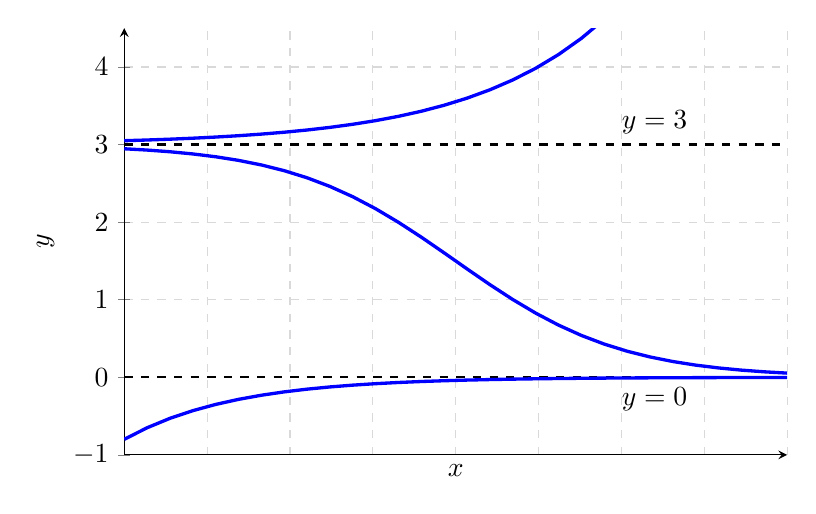
\begin{tikzpicture}
                \begin{axis}[
                    xmajorticks=false,
                    domain=0:4,
                    xmin=0, xmax=4,
                    ymin=-1, ymax=4.5,
                    xlabel=$x$, ylabel=$y$,
                    axis lines=left,
                    grid=both,
                    grid style={dashed, gray!30},
                    width=10cm, height=7cm,
                    restrict y to domain=-1:5
                ]
                
                % Retas de Equilíbrio
                \addplot [black, dashed, thick, domain=0:4] {3} node[pos=0.8, above] {$y=3$};
                \addplot [black, dashed, thick, domain=0:4] {0} node[pos=0.8, below] {$y=0$};
                
                % Curvas Integrais (Azul)
                \addplot [blue, very thick, samples=30, domain=0:4] {3 + 0.05*exp(1.2*x)}; % Região y > 3
                \addplot [blue, very thick, samples=30, domain=0:4] {3 / (1 + exp(2*(x-2)))}; % Região 0 < y < 3
                \addplot [blue, very thick, samples=30, domain=0:4] {-0.8*exp(-1.5*x)}; % Região y < 0
                \end{axis}
            \end{tikzpicture}
        \end{figure}

        \itemresolucao Igualando $f(y)$ a zero para encontrar as soluções de equilíbrio, temos
        \[ (y - 2)^4 = 0 \implies y = 2 \]

        Além disso, como a potência é par, $(y - 2)^4 \geq 0$ para todo $y$. A derivada não muda de sinal nas proximidades do ponto crítico, sendo sempre positiva. Dessa maneira, construímos o retrato de fase e classificamos o ponto de equilíbrio:
        \begin{figure}[H]
            \centering
            \begin{tikzpicture}[scale=0.5]                
                \draw[axis] (0,-2) -- (0,5);
                
                \node[dot, label=right:{$y=2$ (Semiestável)}] at (0,2) {};
                
                % Região y < 2 (Sobe)
                \foreach \y in {-1.6, -0.6, 0.4, 1.4} 
                    \draw[dir] (0, \y) -- (0, \y+0.4);
                    
                % Região y > 2 (Sobe)
                \foreach \y in {2.4, 3.4, 4.4} 
                    \draw[dir] (0, \y) -- (0, \y+0.4);
            \end{tikzpicture}
        \end{figure}
        Assim, podemos esboçar as curvas integrais típicas para as duas regiões do plano:
        \begin{figure}[H]
            \centering
            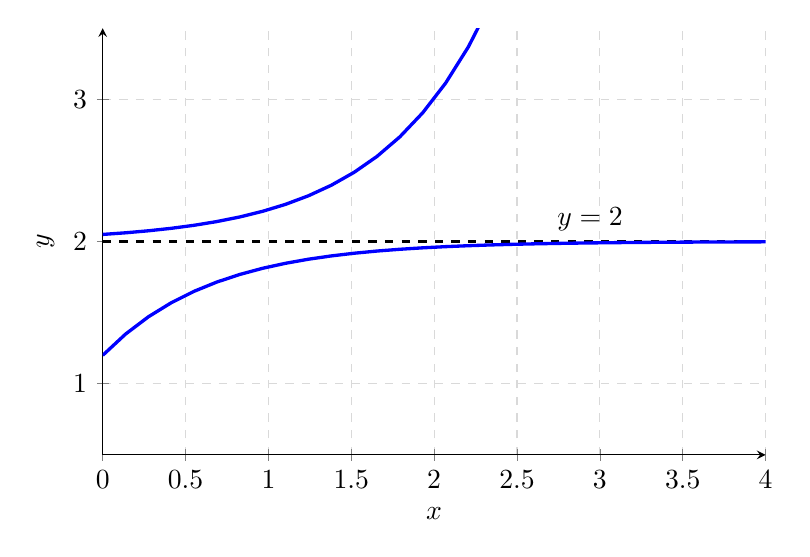
\begin{tikzpicture}
                \begin{axis}[
                    domain=0:4,
                    xmin=0, xmax=4,
                    ymin=0.5, ymax=3.5,
                    xlabel=$x$, ylabel=$y$,
                    axis lines=left,
                    grid=both,
                    grid style={dashed, gray!30},
                    width=10cm, height=7cm,
                    restrict y to domain=0:4
                ]
                
                % Retas de Equilíbrio
                \addplot [black, dashed, thick, domain=0:4] {2} node[pos=0.8, above left] {$y=2$};
                
                % Curvas Integrais (Azul)
                \addplot [blue, very thick, samples=30, domain=0:4] {2 + 0.05*exp(1.5*x)}; % Região y > 2
                \addplot [blue, very thick, samples=30, domain=0:4] {2 - 0.8*exp(-1.5*x)}; % Região y < 2
                \end{axis}
            \end{tikzpicture}
        \end{figure}

        \itemresolucao Igualamos a expressão de $f(y)$ a zero:
        \[ \frac{ye^y - 9y}{e^y} = 0 \implies ye^y - 9y = 0 \]

        Fatorando a expressão, obtemos $y(e^y - 9) = 0$. Ou seja, os pontos críticos são $y = 0$ e $y = \ln(9)$. Além disso, analisando o sinal de $\dfrac{dy}{dx}=f(y)$, temos que
        \[\begin{cases}
            \dfrac{dy}{dx}>0,\quad y<0\\
            \dfrac{dy}{dx}<0,\quad 0<y<\ln(9)\\
            \dfrac{dy}{dx}>0,\quad y>\ln(9)\\
        \end{cases}\]
        Dessa maneira, traçamos o retrato de fase da equação diferencial e classificamos os pontos críticos.
        \begin{figure}[H]
            \centering
            \begin{tikzpicture}[scale=0.5]

                \draw[axis] (0,-2) -- (0,5);
                
                \node[dot, label=right:{$y=\ln(9)$ (Instável)}] at (0,2.197) {};
                \node[dot, label=right:{$y=0$ (Assintoticamente estável)}] at (0,0) {};
                
                % Região y < 0 (Sobe)
                \foreach \y in {-1.8, -1.0} 
                    \draw[dir] (0, \y) -- (0, \y+0.4);
                    
                % Região 0 < y < ln(9) (Desce)
                \foreach \y in {1.6, 0.8} 
                    \draw[dir] (0, \y) -- (0, \y-0.4);
                    
                % Região y > ln(9) (Sobe)
                \foreach \y in {2.6, 3.4, 4.2} 
                    \draw[dir] (0, \y) -- (0, \y+0.4);
            \end{tikzpicture}
        \end{figure}
        Por fim, podemos esboçar as curvas típicas para cada uma das regiões definidas pelos pontos críticos.
        \begin{figure}[H]
            \centering
            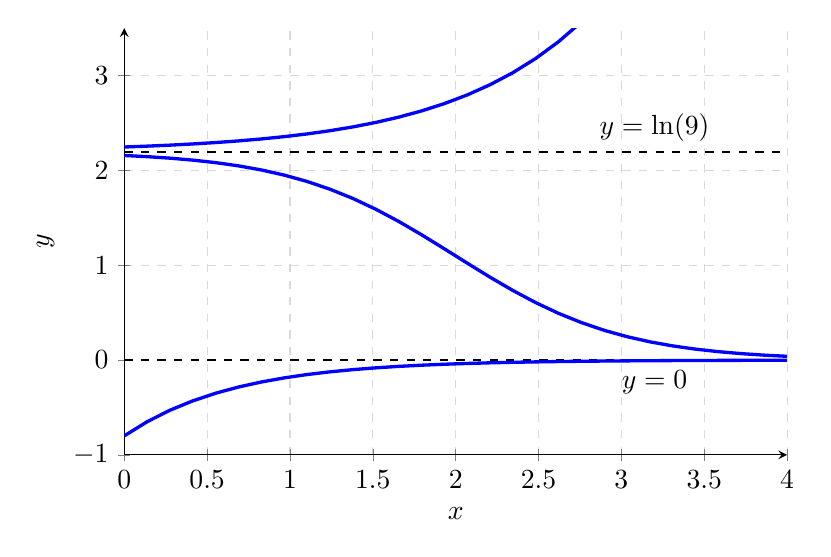
\begin{tikzpicture}
                \begin{axis}[
                    domain=0:4,
                    xmin=0, xmax=4,
                    ymin=-1, ymax=3.5,
                    xlabel=$x$, ylabel=$y$,
                    axis lines=left,
                    grid=both,
                    grid style={dashed, gray!30},
                    width=10cm, height=7cm,
                    restrict y to domain=-1.5:4
                ]
                
                % Retas de Equilíbrio
                \addplot [black, dashed, thick, domain=0:4] {2.1972} node[pos=0.8, above] {$y=\ln(9)$};
                \addplot [black, dashed, thick, domain=0:4] {0} node[pos=0.8, below] {$y=0$};
                
                % Curvas Integrais (Azul)
                \addplot [blue, very thick, samples=30, domain=0:4] {2.1972 + 0.05*exp(1.2*x)}; % Região y > ln(9)
                \addplot [blue, very thick, samples=30, domain=0:4] {2.1972 / (1 + exp(2*(x-2)))}; % Região 0 < y < ln(9)
                \addplot [blue, very thick, samples=30, domain=0:4] {-0.8*exp(-1.5*x)}; % Região y < 0
                \end{axis}
            \end{tikzpicture}
        \end{figure}
    \end{resolucao}

    \begin{resolucao}
        \itemresolucao A equação diferencial dada pode ser reescrita da seguinte forma, separando as variáveis:
        \[e^xy\frac{dy}{dx}=e^{-y}(1+e^{-2x})\Rightarrow ye^ydy=e^{-x}+e^{-3x}dx\]
        Integrando ambos os lados,
        \[\int ye^ydy=\int e^{-x}+e^{-3x}dx\Rightarrow ye^y-e^y=-e^{-x}-\frac{e^{-3x}}{3}+C\]
        Ou seja, uma solução implícita da equação diferencial dada é
        \[\boxed{e^y(y-1)=-e^{-x}-\frac{e^{-3x}}{3}+C}\]

        \itemresolucao Reescrevendo a equação diferencial dada,
        \[\frac{dy}{(2y+3)^2}=\frac{dx}{(4x+5)^2}\]
        Integrando ambos os lados,
        \[\int\frac{dy}{(2y+3)^2}=\int\frac{dx}{(4x+5)^2}\]
        Fazemos as seguintes mudanças de variáveis:
        \[\begin{cases}
            u=2y+3\Rightarrow du=2dy\\
            v=4x+5\Rightarrow dv=4dx\\
        \end{cases}\]
        Dessa maneira,
        \[\frac{1}{2}\int\frac{du}{u^2}=\frac{1}{4}\int\frac{dv}{v^2}\Rightarrow\frac{1}{2}\left(-\frac{1}{u}\right)=\frac{1}{4}\left(-\frac{1}{v}\right)+C_1\]
        \[\frac{1}{2y+3}=\frac{1}{2(4x+5)}+C,\quad\text{onde }C=-C_1\]
        Isolando y para determinar uma solução explícita, 
        \[\boxed{y=\frac{(8-24C)x+7-30C}{16Cx+20C+2}}\]

        \itemresolucao Manipulando a equação diferencial fornecida, temos
        \[\frac{1}{\sin(y)}dx=-\frac{1}{\cos^2(x)}dy\Rightarrow-\cos^2(x)dx=\sin(y)dy\]
        \[-\int\cos^2(x)dx=\int\sin(y)dy\]
        A integração do lado direito da equação é direta. Desenvolvendo a integral do lado esquerdo por partes (note que ela também pode ser resolvida pela manipulação de $\cos(2x)=2\cos^2(x)-1$), adotamos
        \[\begin{cases}
            u=\cos(x)\rightarrow du=-\sin(x)dx\\
            dv=\cos(x)dx\rightarrow v=\sin(x)dx
        \end{cases}\]
        Dessa maneira,
        \[\int\cos^2(x)dx=\sin(x)\cos(x)+\int \sin^2(x)dx=\sin(x)\cos(x)+\int 1-\cos^2(x)dx\]
        \[\int\cos^2(x)dx=\sin(x)\cos(x)+\int dx-\int\cos^2(x)dx\]
        Agrupando as integrais de $\cos^2(x)$,
        \[2\int\cos^2(x)dx=\sin(x)\cos(x)+x\Rightarrow \int\cos^2(x)dx=\frac{\sin(x)\cos(x)}{2}+\frac{x}{2}\]
        Retornando à equação diferencial dada,
        \[-\cos(y)+C=-\frac{\sin(x)\cos(x)}{2}+\frac{x}{2}\Rightarrow\boxed{y=\arccos\left(\frac{\sin(x)\cos(x)+x}{2}-C\right)}\]

        \itemresolucao Reescrevendo a equação diferencial,
        \[(e^y+1)^2e^{-y}dx=-e^{-x}(e^x+1)^3dy\Rightarrow\frac{e^x}{(e^x+1)^3}dx=-\frac{e^y}{(e^y+1)^2}dy\]
        Antes de integrar ambos os lados, façamos as seguintes substituições:
        \[\begin{cases}
            u=e^y+1\rightarrow du=e^ydy\\
            v=e^x+1\rightarrow dv=e^xdx\\
        \end{cases}\]
        Dessa maneira, temos
        \[\int\frac{dv}{v^3}=-\int\frac{du}{u^2}\Rightarrow-\frac{1}{2v^2}+C=\frac{1}{u}\Rightarrow\frac{2v^2C-1}{2v^2}=\frac{1}{u}\Rightarrow u=\frac{2v^2}{2v^2C-1}\]
        Por fim, substituindo os valores,
        \[e^y+1=\frac{2(e^x+1)^2}{2(e^x+1)^2C-1}\Rightarrow\boxed{y=\ln\left(\frac{2(e^x+1)^2}{2(e^x+1)^2C-1}-1\right)}\]

        \itemresolucao Podemos reescrever a equação da seguinte forma: \[\frac{dP}{P(1-P)}=dt\Rightarrow\frac{dP}{P}+\frac{dP}{1-P}=dt\]
        Integrando ambos os lados da equação, obtemos
        \[\ln|P|-\ln|1-P|=t+C_1\Rightarrow\ln\left|\frac{P}{1-P}\right|=t+C_1\Rightarrow\left|\frac{P}{1-P}\right|=C_2e^t\]
        onde $C_2=e^{C_1}$. Retirando o módulo,
        \[\frac{P}{1-P}=\pm C_2e^t=Ce^t\]
        já que $C$ é uma constante arbitrária e pode assumir qualquer sinal. Por fim, isolando $P$, obtemos
        \[\boxed{P=\frac{Ce^t}{1+Ce^t}}\]

        \itemresolucao Separando os termos da equação,
        \[\frac{dy}{\sqrt{1-y^2}}=xdx\Rightarrow\int\frac{dy}{\sqrt{1-y^2}}=\int xdx\]
        Para integrar o lado esquerdo da equação, fazemos a seguinte substituição de variáveis:
        \[\begin{cases}
            y=\sin(\theta)\\
            dy=\cos(\theta)d\theta
        \end{cases}\]
        Dessa forma,
        \[\int \frac{\cos(\theta)}{\sqrt{1-\sin^2(\theta)}}d\theta=\int \frac{\cos(\theta)}{\sqrt{\cos^2(\theta)}}d\theta=\int \frac{\cos(\theta)}{\cos(\theta)}d\theta=\theta,\quad-\frac{\pi}{2}\leq\theta\leq\frac{\pi}{2}\]
        Pela substituição previamente realizada, sabemos, portanto, que o resultado da integral é $\theta=\arcsin(y)$. Substituindo na equação diferencial,
        \[\arcsin(y)=\frac{x^2}{2}+C\Rightarrow \boxed{y=\sin\left(\frac{x^2}{2}+C\right)}\]

    \end{resolucao}

    \begin{resolucao}
        Separando as variáveis da equação diferencial dada, \[\frac{2x}{x^2+10}dx=\frac{\cos(y)}{\sin^2(y)}dy\Rightarrow\int\frac{2x}{x^2+10}dx=\int\frac{\cos(y)}{\sin^2(y)}dy\]
        Façamos as seguintes mudanças de variável:
        \[\begin{cases}
            u=x^2+10\rightarrow du=2xdx\\
            v=\sin(y)\rightarrow dv=\cos(y)dy
        \end{cases}\]
        Dessa forma,
        \[\int\frac{du}{u}=\frac{dv}{v^2}\Rightarrow\ln|u|=-\frac{1}{v}+C\Rightarrow\ln|x^2+10|=-\frac{1}{\sin(y)}+C\]
        Como $x^2+10$ é sempre positivo, podemos retirar o módulo. Dessa forma, chegamos à expressão do enunciado, $\boxed{\ln(x^2+10)+\mathrm{cossec}(y)=C}$.

        A fim de encontrar as soluções constantes da EDO, podemos reorganizá-la na forma
        \[\frac{dy}{dx}=\frac{2x}{x^2+10}\frac{\sin^2(y)}{\cos(y)}=0\Rightarrow2x\sin^2(y)=0\Rightarrow\boxed{y=k\pi,~k\in\mathbb{Z}}\]
    \end{resolucao}

    \begin{resolucao}
        \itemresolucao Separando as variáveis, temos
        \[ydy=e^{\sqrt{x}}dx\Rightarrow\int ydy=\int e^{\sqrt{x}}dx\]
        Para resolver a integral do lado direito, podemos realizar a seguinte mudança de variáveis:
        \[
            u=x^{\frac{1}{2}}\rightarrow du=\frac{1}{2}x^{-\frac{1}{2}}dx\Rightarrow dx=2x^{\frac{1}{2}}du=2udu
        \]
        Portanto, a equação diferencial se torna
        \[\frac{y^2}{2}=\int e^u2udu\Rightarrow\frac{y^2}{4}=ue^u-e^u+C\]
        \[\frac{y^2}{4}=e^{\sqrt{x}}(\sqrt{x}-1)+C\Rightarrow y=\pm\sqrt{4e^{\sqrt{x}}(\sqrt{x}-1)+C}\]
        Tomamos a equação de sinal positivo, pois dada a condição inicial fornecida, $y(x)$ deve assumir valores positivos. Substituindo a CI para determinar a constante de integração,
        \[4=\sqrt{4e\cdot0+C}\Rightarrow C=16\]
        Assim, obtemos a solução da equação diferencial:
        \[\boxed{y(x)=\sqrt{4e^{\sqrt{x}}(\sqrt{x}-1)+16}}\]

        \itemresolucao Reescrevendo a equação diferencial,
        \[ydy=x\arctan(x)dx\Rightarrow\int ydy=\int x\arctan(x)dx\]
        Podemos integrar o lado direito da equação por partes. Tomemos
        \[\begin{cases}
            u=\arctan(u)\rightarrow du=\dfrac{1}{x^2+1}dx\\
            dv=xdx\rightarrow v=\dfrac{x^2}{2}
        \end{cases}\]
        Dessa maneira,
        \[\int x\arctan(x)dx=\frac{x^2}{2}\arctan(x)-\frac{1}{2}\int\frac{x^2}{x^2+1}dx \]
        Podemos desenvolver a integral de $\dfrac{x^2}{x^2+1}$ da seguinte forma:
        \[\int\frac{x^2}{x^2+1}dx=\int\frac{x^2+1-1}{x^2+1}dx=\int\frac{x^2+1}{x^2+1}dx-\int\frac{1}{x^2+1}dx\]
        \[\int\frac{x^2}{x^2+1}dx=x-\arctan(x)+C\]
        Portanto, 
        \[\int x\arctan(x)dx=\frac{x^2}{2}\arctan(x)-\frac{1}{2}(x-\arctan(x)+C)\]
        Substituindo na equação diferencial,
        \[\frac{y^2}{2}=\frac{x^2}{2}\arctan(x)-\frac{1}{2}(x-\arctan(x)+C)\]
        \[y^2=(x^2+1)\arctan(x)-x-C\Rightarrow y=\pm\sqrt{(x^2+1)\arctan(x)-x-C}\]
        Dada a condição inicial positiva, tomamos a expressão de $y$ que retorna valores positivos. Substituindo a CI em $y$, temos
        \[3=\sqrt{-C}\Rightarrow -C=9\]
        Dessa maneira,
        \[\boxed{y(x)=\sqrt{(x^2+1)\arctan(x)-x+9}}\]

    \end{resolucao}

    \begin{resolucao}
        \itemresolucao Dada a equação diferencial, temos que $P(x)=1$. Dessa maneira, $\mu(x)=e^{\int P(x)dx}=e^{\int dx}e^{x}$. Multiplicando o fator integrante encontrado em ambos os lados da ED,
        \[e^x\frac{dy}{dx}+e^xy=e^{4x}\Rightarrow \frac{d}{dx}(ye^x)=e^{4x}\Rightarrow \int\frac{d}{dx}(ye^x)dx=\int e^{4x}dx\]
        \[ye^x=\frac{e^{4x}}{4}+C\Rightarrow \boxed{y(x)=Ce^{-x}+\frac{e^{3x}}{4}}\]
        O termo $Ce^{-x}$ é transiente, dado que $e^{-x}\to0$ quando $x\to\infty$. Tanto a ED quanto a solução geral são definidas para todo $x\in\mathbb{R}$. Portanto, tomamos o intervalo como $I=(\infty, \infty)$.

        \itemresolucao Podemos reorganizar a equação diferencial da seguinte forma:
        \[\frac{dy}{dx}-\frac{x}{1+x}y=\frac{x(1+x)}{1+x}\Rightarrow\frac{dy}{dx}-\frac{x}{1+x}y=x\]
        Assim, identificamos $P(x)=-\dfrac{x}{1+x}$. A fim de integrar esse fator, somamos e subtraímos 1 no numerador:
        \[-\int\frac{x}{1+x}dx=-\int\frac{x+1-1}{1+x}dx=-\left[\int dx-\int\frac{1}{1+x}dx\right]\]
        \[-\int\frac{x}{1+x}dx=-x+\ln|1+x|\]
        Dessa forma, $\mu(x)=e^{\int P(x)dx}=e^{-x}e^{\ln|1+x|}=|1+x|e^{-x}$. Ou, como o fator integrante multiplica os dois lados da equação, $\mu(x)=(1+x)e^{-x}$, já que o sinal é anulado. Multiplicando ambos os lados da equação diferencial,
        \[\frac{d}{dx}(y(1+x)e^{-x})=(x+x^2)e^{-x}\]
        A fim de integrar o lado direito, fazemos a seguinte mudança de variáveis:
        \[\begin{cases}
            u=x^2+x\rightarrow du=(2x+1)dx\\
            dv=e^{-x}dx\rightarrow v=-e^{-x}
        \end{cases}\]
        Assim,
        \[\int (x+x^2)e^{-x}dx=-(x^2+x)e^{-x}+\int e^{-x}(2x+1)dx=-(x^2+x)e^{-x}+\int 2xe^{-x}+e^{-x}dx\]
        \[\int (x+x^2)e^{-x}dx=-(x^2+x)e^{-x}+2(-xe^{-x}-e^{-x})-e^{-x}+C\]
        \[\int (x+x^2)e^{-x}dx=-e^{-x}(x^2+3x+3)+C\]
        Ou seja,
        \[y(1+x)e^{-x}=-e^{-x}(x^2+3x+3)+C\Rightarrow \boxed{y(x)=\frac{Ce^{x}}{1+x}-\frac{x^2+3x+3}{1+x}}\]
        Tanto a solução encontrada quanto a equação diferencial na forma padrão não são definidas para $x=-1$. Dessa forma, tomamos $I=(-1,\infty)$ como o maior intervalo de definição. Não há termos transientes.

        \itemresolucao Dividindo ambos os lados da equação por $x$
        \[y'+\frac{1+x}{x}y=\frac{e^{-x}\sin(2x)}{x}\]
        Dessa maneira, o fator integrante é dado por
        \[\mu(x)=e^{\int \frac{x+1}{x}dx}=e^{x+\ln|x|}=|x|e^x\]
        Ou, considerando que o fator multiplica ambos os lados da equação, $\mu(x)=xe^x$. Realizando esse passo e integrando ambos os lados,
        \[\int\frac{d}{dx}(yxe^x)dx=\int\sin(2x)dx\Rightarrow yxe^x=\frac{-\cos(2x)}{2}+C\]
        \[\boxed{y(x)=\frac{-e^{-x}\cos(2x)}{2x}+\frac{Ce^{-x}}{x}}\]
        Analisando a equação diferencial na forma padrão e a solução obtidas, observa-se que nenhuma das duas é definida para $x=0$. Dessa forma, podemos tomar $I=(0, \infty)$ como o maior intervalo de definição. Ademais, como $e^{-x}$ aparece em ambos os termos da solução, dizemos que esta é transiente (ou seja, tende a $0$ quando $x\to\infty$).

        \itemresolucao A equação diferencial já está organizada na forma padrão. Assim, temos $P(\theta)=\sec(\theta)$. Integrando esse termo em relação a $\theta$, temos
        \[\int \sec(\theta)d\theta=\int\sec(\theta)\frac{\sec(\theta)+\tan(\theta)}{\sec(\theta)+\tan(\theta)}d\theta=\int\frac{\sec^2(\theta)+\sec(\theta)\tan(\theta)}{\sec(\theta)+\tan(\theta)}d\theta\]
        Com isso, fazemos a seguinte mudança de variáveis: 
        \[\begin{cases}
            u=\sec(\theta)+\tan(\theta)\\
            du=\sec^2(\theta)+\sec(\theta)\tan(\theta)d\theta
        \end{cases}\]
        Portanto,
        \[\int \sec(\theta)d\theta=\int\frac{du}{u}=\ln|u|=\ln|\sec(\theta)+\tan(\theta)|\]
        Dessa maneira, o fator integrante é $\mu(x)=e^{\ln|\sec(\theta)+\tan(\theta)|}=\sec(\theta)+\tan(\theta)$
        Multiplicando e integrando ambos os lados da equação diferencial,
        \[(\sec(\theta)+\tan(\theta))r=\int 1+\sin(\theta)d\theta=\theta-\cos(\theta)+C\]
        \[\boxed{r(\theta)=\frac{\theta-\cos(\theta)+C}{\sec(\theta)+\tan(\theta)}}\]
        A equação diferencial é indefinida em $\mathbb{R}$ quando $\cos(\theta)=0$. Ou seja, $\theta\neq\dfrac{(2k+1)\pi}{2},~k\in\mathbb{Z}$. Além disso, o denominador da solução encontrada deve ser diferente de $0$ e $\theta$ deve satisfazer os intervalos de definição das funções trigonométricas, condição também satisfeita por $\theta\neq\dfrac{(2k+1)\pi}{2},~k\in\mathbb{Z}$. Assim, tomamos o maior intervalo de definição como $I=\left(-\dfrac{\pi}{2}, \dfrac{\pi}{2}\right)$.
    \end{resolucao}

    \begin{resolucao}
        Primeiramente, devemos encontrar o fator integrante. Como $P(x)=2$, $\mu(x)=e^{2x}$. Multiplicando e integrando ambos os lados da equação, temos
        \[ye^{2x}=\int e^{2x}f(x)dx\]
        Substituindo $f(x)=1$, podemos determinar
        \[ye^{2x}=\int e^{2x}dx=\frac{e^{2x}}{2}+C\Rightarrow y(x)=Ce^{-2x}+\frac{1}{2},~0\leq x\leq3\]
        Substituindo a condição inicial, $C=-\dfrac{1}{2}$. Portanto,
        \[y(x)=\frac{1-e^{-2x}}{2},~0\leq x\leq3\]
        Agora, substituímos $f(x)=0$ na expressão previamente encontrada. Com isso, calculamos
        \[ye^{2x}=\int dx=C\Rightarrow y=Ce^{-2x},~x>3\]
        Usamos o fato de que a função deve ser contínua em $x=3$ para encontrar o valor da constante de integração:
        \[\frac{1-e^{-2\cdot3}}{2}=Ce^{-2\cdot3}\Rightarrow C=\frac{e^6-1}{2}\]
        Ou seja, $y(x)=\dfrac{e^6-1}{2}e^{-2x},~x>3$. Assim, a função que resolve o PVI dado é
        \begin{gather*}
            \boxed{
            y(x)=\begin{cases}
                \dfrac{1-e^{-2x}}{2},\quad0\leq x\leq3\\
                \dfrac{e^6-1}{2}e^{-2x},\quad x>3
            \end{cases}
            }
        \end{gather*}
        O plot da função pode ser observado abaixo:
        \begin{figure}[H]
            \centering
            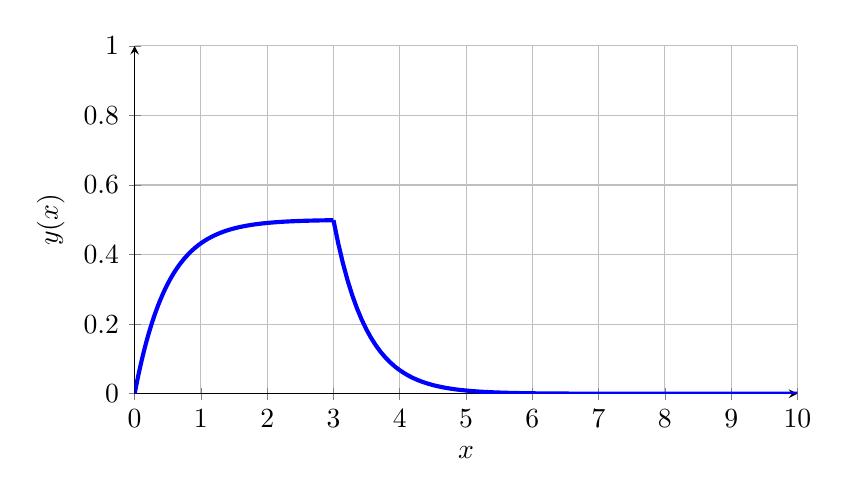
\begin{tikzpicture}
                \begin{axis}[
                    axis lines = left,
                    xlabel = {$x$},
                    ylabel = {$y(x)$},
                    ymin = 0, ymax = 1, % Ajuste os limites de y conforme necessário
                    xmin = 0, xmax = 10, 
                    grid = major,
                    width = 10cm,
                    height = 6cm,
                    samples = 100,
                    xtick = {0, 1,...,10},
                    ytick = {0, 0.2,...,1}
                    %legend pos = north east
                ]

                % Primeira parte da função: 0 <= x <= 3
                \addplot [
                    domain=0:3,
                    color=blue,
                    line width=1.5
                ]
                {(1 - exp(-2*x))/2};

                % Segunda parte da função: x > 3
                \addplot [
                    domain=3:10, % Limite superior arbitrário (6) para visualização
                    color=blue,
                    line width = 1.5
                ]
                {((exp(6) - 1)/2) * exp(-2*x)};

                \end{axis}
                \end{tikzpicture}
        \end{figure}
    \end{resolucao}

    \begin{resolucao}
        Temos que $P(x)=e^x$. Portanto, o fator integrante da equação diferencial será $\mu(x)=e^{e^x}$. Multiplicando ambos os lados da equação quando $f(x)=1$, temos
        \[\frac{d}{dx}ye^{e^x}=e^{e^x}\]
        Ao tentar integrar ambos os lados, notamos que $\int e^{e^x}dx$ é uma integral não elementar. Dessa forma, utilizaremos integrais definidas na variável auxiliar $t$ para expressar a solução do problema, em que $x>0$:
        \[\int_{0}^{x}\frac{d}{dt}y(t)e^{e^t}dt=\int_{0}^{x}e^{e^t}dt\Rightarrow y(x)e^{e^x}-y(0)e^{e^0}=\int_{0}^{x}e^{e^t}dt\]
        Ou seja,
        \[y(x)=y(0)e^{1-e^x}+e^{-e^x}\int_{0}^{x}e^{e^t}dt\]
        Ou, substituindo a condição inicial,
        \[\boxed{y(x)=e^{1-e^x}+e^{-e^x}\int_{0}^{x}e^{e^t}dt}\]
        Agora, para $f(x)=0$, temos
        \[\int\frac{d}{dx}(ye^{e^x})dx=\int 0dx\Rightarrow ye^{e^x}=C\Rightarrow y=Ce^{-e^x}\]
        Substituindo a condição inicial, $C=e$. Portanto, $\boxed{y(x)=e^{1-e^x}}$.
        Por fim, para $f(x)=e^x$, temos
        \[\frac{d}{dx}ye^{e^x}=e^{x+e^x}\Rightarrow\int\frac{d}{dx}(ye^{e^x})dx=\int e^{x+e^x}dx\]
        Fazendo a mudança de variáveis $u=e^x$, $du=e^xdx$, desenvolvemos
        \[ye^{e^x}=\int e^udu=e^u+C=e^{e^x}+C\]
        \[y(x)=Ce^{-e^x}+1\]
        Substituindo a condição inicial, $C=0$. Portanto, a solução é simplesmente $\boxed{y(x)=1}$
    \end{resolucao}

    \begin{resolucao}
        \itemresolucao Para que a equação seja exata, $\dfrac{\partial M}{\partial y}=\dfrac{\partial N}{\partial x}$. Assim, analisemos as derivadas parciais:
        \[\frac{\partial M}{\partial y}=\frac{\partial}{\partial y}(y\ln(y)-e^{-xy})=\ln(y)+1+xe^{-xy}\]
        \[\frac{\partial N}{\partial x}=\frac{\partial}{\partial x}\left(\frac{1}{y}+x\ln(y)\right)=\ln(y)\]
        Como $\dfrac{\partial M}{\partial y}\neq\dfrac{\partial N}{\partial x}$, a equação fornecida não é exata.

        \itemresolucao Reorganizando a equação diferencial dada,
        \[\left(x^2y^3-\frac{1}{1+9x^2}\right)dx+x^3y^2dy=0\]
        Analisando as derivadas parciais de $M$ e $N$,
        \[\frac{\partial M}{\partial y}=\frac{\partial}{\partial y}\left(x^2y^3-\frac{1}{1+9x^2}\right)=3x^2y^2\]
        \[\frac{\partial N}{\partial x}=\frac{\partial}{\partial x}(x^3y^2)=3x^2y^2\]
        Portanto, a equação é exata. Para resolvê-la, integramos $N$ em relação a $y$:
        \[f(x,y)=\int Ndy=\int x^3y^2dy=\frac{x^3y^3}{3}+g(x)\]
        Derivando em relação a $x$, 
        \[\frac{\partial f}{\partial x}=M=x^2y^3+g'(x)\Rightarrow g'(x)=-\frac{1}{1+9x^2}\]
        Integrando $g'(x)$, fazemos a seguinte mudança de variáveis: $3x=u\rightarrow dx=du/3$. Dessa maneira,
        \[\int g'(x)dx=-\frac{1}{3}\int \frac{du}{1+u^2}=-\frac{1}{3}\arctan(3x)\]
        Assim, encontramos $f(x,y)=c$ que satisfaz a equação diferencial:
        \[\boxed{\frac{x^3y^3}{3}-\frac{1}{3}\arctan(3x)=c}\]

        \itemresolucao Para a equação $(\tan(x)-\sin(x)\sin(y))dx+\cos(x)\cos(y)dy=0$, identificamos as funções $M(x,y)=\tan(x)-\sin(x)\sin(y)$ e $N(x,y)=\cos(x)\cos(y)$. 
        Para verificar se a equação é exata, calculamos as derivadas parciais:
        \[\frac{\partial M}{\partial y}=-\sin(x)\cos(y)\]
        \[\frac{\partial N}{\partial x}=-\sin(x)\cos(y)\]
        Como $\dfrac{\partial M}{\partial y}=\dfrac{\partial N}{\partial x}$, a equação é de fato exata. Para resolvê-la, integramos $N$ em relação a $y$:
        \[f(x,y)=\int\cos(x)\cos(y)dy=\cos(x)\sin(y)+g(x)\]
        Derivando esse resultado em relação a $x$ e igualando a $M$, temos:
        \[\frac{\partial f}{\partial x}=-\sin(x)\sin(y)+g'(x)=\tan(x)-\sin(x)\sin(y)\]
        Logo, concluímos que $g'(x)=\tan(x)$, o que nos fornece $g(x)=\int\tan(x)dx=-\ln|\cos(x)|$. Portanto, a solução da equação diferencial é dada implicitamente por:
        \[\boxed{\cos(x)\sin(y)-\ln|\cos(x)|=c}\]

        \itemresolucao Reorganizando a equação dada para a forma diferencial, obtemos $(2y\sin(x)\cos(x)-y+2y^2e^{xy^2})dx+(-x+\sin^2(x)+4xye^{xy^2})dy=0$. Identificamos $M$ e $N$:
        \[M=2y\sin(x)\cos(x)-y+2y^2e^{xy^2}\]
        \[N=-x+\sin^2(x)+4xye^{xy^2}\]
        Analisando as derivadas parciais:
        \[\frac{\partial M}{\partial y}=2\sin(x)\cos(x)-1+4ye^{xy^2}+4xy^3e^{xy^2}\]
        \[\frac{\partial N}{\partial x}=-1+2\sin(x)\cos(x)+4ye^{xy^2}+4xy^3e^{xy^2}\]
        Como as derivadas parciais são iguais, a equação é exata. Integrando $N$ em relação a $y$:
        \[f(x,y)=\int\left(-x+\sin^2(x)+4xye^{xy^2}\right)dy=-xy+y\sin^2(x)+2e^{xy^2}+g(x)\]
        Derivando em relação a $x$ e igualando a $M$:
        \[\frac{\partial f}{\partial x}=-y+2y\sin(x)\cos(x)+2y^2e^{xy^2}+g'(x)\]
        Assim, concluímos que $g'(x)=0$, o que implica $g(x)=C_1$. Portanto, a solução implícita geral pode ser expressa como:
        \[\boxed{y\sin^2(x)-xy+2e^{xy^2}=c}\]
    \end{resolucao}

    \begin{resolucao}
        \itemresolucao Reescrevendo a equação diferencial na forma $Mdt+Ndy=0$, obtemos:
        \[\left(\frac{t}{2y^4}\right)dt+\left(\frac{3y^2-t^2}{y^5}\right)dy=0\]
        Calculamos as derivadas parciais para verificar se a equação é exata:
        \[\frac{\partial M}{\partial y}=\frac{\partial}{\partial y}\left(\frac{t}{2}y^{-4}\right)=-2ty^{-5}=-\frac{2t}{y^5}\]
        \[\frac{\partial N}{\partial t}=\frac{\partial}{\partial t}\left(3y^{-3}-t^2y^{-5}\right)=-2ty^{-5}=-\frac{2t}{y^5}\]
        A equação é exata. Integrando $M$ em relação a $t$:
        \[f(t,y)=\int \frac{t}{2y^4}dt=\frac{t^2}{4y^4}+g(y)\]
        Derivando em relação a $y$ e igualando a $N$:
        \[\frac{\partial f}{\partial y}=-\frac{t^2}{y^5}+g'(y)=\frac{3y^2-t^2}{y^5}=\frac{3}{y^3}-\frac{t^2}{y^5}\]
        Disso, extraímos que $g'(y)=\dfrac{3}{y^3}$, o que nos dá $g(y)=\int 3y^{-3}dy=-\dfrac{3}{2y^2}$.
        A família de soluções a um parâmetro é $\dfrac{t^2}{4y^4}-\dfrac{3}{2y^2}=C$. Usando a condição inicial do PVI, $y(1)=1$:
        \[\frac{1^2}{4(1)^4}-\frac{3}{2(1)^2}=C\implies C=\frac{1}{4}-\frac{6}{4}=-\frac{5}{4}\]
        Multiplicando toda a equação por $4$, a solução do Problema de Valor Inicial é dada por:
        \[\boxed{\frac{t^2}{y^4}-\frac{6}{y^2}=-5}\]

        \itemresolucao Reescrevendo a equação diferencial,
        \[(y^2+y\sin(x))dx+\left(2xy-\frac{1}{1+y^2}+\cos(x)\right)=0\]
        Dessa forma,
        \[\frac{\partial M}{\partial y}=\frac{\partial}{\partial y}(y^2+y\sin(x))=2y+\sin(x)\]
        \[\frac{\partial N}{\partial x}=\frac{\partial}{\partial x}\left(2xy-\frac{1}{1+y^2}-\cos(x)\right)=2y+\sin(x)\]
        Assim, conclui-se que a equação é exata. Integrando $M$ em relação a $x$,
        \[f(x,y)=\int y^2+y\sin(x)dx=y^2x-y\cos(x)+g(y)\]
        Derivando em relação a $y$,
        \[\frac{\partial f}{\partial y}=N=2xy-\cos(x)+g'(y)\]
        Ou seja, $g'(y)=-\dfrac{1}{1+y^2}$ e, portanto, $g(y)=-\arctan(y)$. Dessa maneira, a família de soluções a um parâmetro é $y^2x-y\cos(x)-\arctan(y)=c$. Substituindo a condição inicial fornecida, $c=-1-\pi/4$. Assim, a solução do PVI é
        \[\boxed{y^2x-y\cos(x)-\arctan(y)=-\left(1+\frac{\pi}{4}\right)}\]
    \end{resolucao}

    \begin{resolucao}
        \itemresolucao A equação diferencial dada é $xdx+(x^2y+4y)dy=0$. Identificamos $M(x,y)=x$ e $N(x,y)=x^2y+4y=y(x^2+4)$.
        Calculando as derivadas parciais, temos:
        \[\frac{\partial M}{\partial y}=0 \quad \text{e} \quad \frac{\partial N}{\partial x}=2xy\]
        Como $\frac{\partial M}{\partial y} \neq \frac{\partial N}{\partial x}$, a equação não é exata. Vamos procurar um fator integrante $\mu$. Calculando a expressão proposta:
        \[\frac{\frac{\partial N}{\partial x}-\frac{\partial M}{\partial y}}{M}=\frac{2xy-0}{x}=2y\]
        Como o resultado depende apenas de $y$, podemos encontrar um fator integrante $\mu(y)$:
        \[\mu(y)=e^{\int 2y dy}=e^{y^2}\]
        Multiplicando a equação original por $\mu(y)$, obtemos a nova equação:
        \[xe^{y^2}dx+y(x^2+4)e^{y^2}dy=0\]
        Esta equação agora é exata. Integrando a nova parcela $M$ em relação a $x$:
        \[f(x,y)=\int xe^{y^2} dx=\frac{x^2}{2}e^{y^2}+g(y)\]
        Derivando em relação a $y$ e igualando à nova parcela $N$:
        \[\frac{\partial f}{\partial y}=\frac{x^2}{2}(2ye^{y^2})+g'(y)=x^2ye^{y^2}+g'(y)\]
        \[x^2ye^{y^2}+g'(y) = y(x^2+4)e^{y^2} = x^2ye^{y^2}+4ye^{y^2}\]
        Isso nos fornece $g'(y)=4ye^{y^2}$. Para integrar e achar $g(y)$, fazemos a substituição $u=y^2$, com $du=2ydy$:
        \[g(y)=\int 4ye^{y^2}dy = 2\int e^{u}du = 2e^{y^2}\]
        A família de soluções a um parâmetro é dada por $\dfrac{x^2}{2}e^{y^2}+2e^{y^2}=C_1$.
        Multiplicando por $2$ e colocando a exponencial em evidência, obtemos a solução implícita:
        \[(x^2+4)e^{y^2}=C\]
        Aplicando a condição inicial do PVI, $y(4)=0$:
        \[(4^2+4)e^{0^2}=C \implies C=20 \cdot 1 = 20\]
        Portanto, a solução do Problema de Valor Inicial é:
        \[(x^2+4)e^{y^2}=20\]
        Ou, na forma explícita,
        \[\boxed{y(x)=\sqrt{\ln\left(\frac{20}{x^2+4}\right)}}\]

        \itemresolucao Reescrevendo a equação diferencial na forma $Mdx+Ndy=0$, obtemos:
        \[(x^2+y^2-5)dx-(y+xy)dy=0\]
        Identificamos $M(x,y)=x^2+y^2-5$ e $N(x,y)=-y(1+x)$.
        Calculando as derivadas parciais:
        \[\frac{\partial M}{\partial y}=2y \quad \text{e} \quad \frac{\partial N}{\partial x}=-y\]
        Como $\frac{\partial M}{\partial y} \neq \frac{\partial N}{\partial x}$, a equação não é exata. Buscamos um fator integrante através da expressão:
        \[\frac{\frac{\partial M}{\partial y}-\frac{\partial N}{\partial x}}{N}=\frac{2y-(-y)}{-y(1+x)}=\frac{3y}{-y(1+x)}=-\frac{3}{1+x}\]
        Como a expressão depende apenas de $x$, o fator integrante $\mu(x)$ é:
        \[\mu(x)=e^{\int -\frac{3}{1+x} dx}=e^{-3\ln|1+x|}=\frac{1}{(1+x)^3}\]
        Multiplicando a equação original por $\mu(x)$, obtemos a equação exata:
        \[\frac{x^2+y^2-5}{(1+x)^3}dx-\frac{y}{(1+x)^2}dy=0\]
        Integrando a nova parcela $N$ em relação a $y$, 
        \[f(x,y)=\int -\frac{y}{(1+x)^2} dy=-\frac{y^2}{2(1+x)^2}+g(x)\]
        Derivando em relação a $x$ e igualando à nova parcela $M$:
        \[\frac{\partial f}{\partial x}=\frac{y^2}{(1+x)^3}+g'(x)=\frac{x^2+y^2-5}{(1+x)^3}=\frac{x^2-5}{(1+x)^3}+\frac{y^2}{(1+x)^3}\]
        Isso nos fornece $g'(x)=\frac{x^2-5}{(1+x)^3}$. Para integrar essa expressão, fazemos a substituição $u=1+x$, o que nos dá $x=u-1$ e $dx=du$:
        \[g(x)=\int \frac{(u-1)^2-5}{u^3} du=\int \frac{u^2-2u-4}{u^3} du=\int \left(\frac{1}{u}-\frac{2}{u^2}-\frac{4}{u^3}\right) du\]
        \[g(x)=\ln|u|+\frac{2}{u}+\frac{2}{u^2}=\ln|1+x|+\frac{2}{1+x}+\frac{2}{(1+x)^2}\]
        A família de soluções a um parâmetro é $-\dfrac{y^2}{2(1+x)^2}+\ln|1+x|+\dfrac{2}{1+x}+\dfrac{2}{(1+x)^2}=C_1$.
        Multiplicando por $2$ e desenvolvendo as frações, temos:
        \[\frac{-y^2+4(1+x)+4}{(1+x)^2}+2\ln|1+x|=C\]
        \[\frac{-y^2+4x+8}{(1+x)^2}+2\ln|1+x|=C\]
        Aplicando a condição inicial $y(0)=1$:
        \[\frac{-(1)^2+4(0)+8}{(0+1)^2}+2\ln|1|=C \implies C=7\]
        Portanto, a solução implícita do PVI é:
        \[\boxed{\frac{-y^2+4x+8}{(1+x)^2}+2\ln|1+x|=7}\]
    \end{resolucao}

    \begin{resolucao}
        \itemresolucao Faremos a substituição $y=ux$, o que implica $dy=udx+xdu$. Substituindo na equação:
        \[((ux)^2+(ux)x)dx+x^2(udx+xdu)=0\]
        \[(u^2x^2+ux^2)dx+x^2(udx+xdu)=0\]
        Dividindo toda a equação por $x^2$ (assumindo $x \neq 0$), obtemos:
        \[(u^2+u)dx+udx+xdu=0 \implies (u^2+2u)dx+xdu=0\]
        Separando as variáveis:
        \[\frac{du}{u^2+2u}=-\frac{dx}{x}\]
        Para integrar o lado esquerdo, utilizamos frações parciais:
        \[\frac{1}{u(u+2)}=\frac{A}{u}+\frac{B}{u+2} \implies 1 = (A+B)+2A \implies A=\frac{1}{2},~B=-\frac{1}{2}\]
        Integrando ambos os lados:
        \[\frac{1}{2}\int\left(\frac{1}{u}-\frac{1}{u+2}\right)du=-\int\frac{dx}{x}\]
        \[\frac{1}{2}(\ln|u|-\ln|u+2|)=-\ln|x|+C_1 \implies \ln\left|\frac{u}{u+2}\right|=-2\ln|x|+2C_1\]
        Aplicando a exponencial em ambos os lados e chamando $C=e^{2C_1}$:
        \[\frac{u}{u+2}=\frac{C}{x^2}\]
        Substituindo $u=\dfrac{y}{x}$ de volta:
        \[\frac{\frac{y}{x}}{\frac{y}{x}+2}=\frac{C}{x^2} \implies \frac{y}{y+2x}=\frac{C}{x^2}\]
        Portanto, a solução implícita é dada por:
        \[\boxed{x^2y=C(y+2x)}\]

        \itemresolucao Usaremos a substituição $y=ux$, o que nos dá $\dfrac{dy}{dx}=u+x\dfrac{du}{dx}$:
        \[u+x\frac{du}{dx}=\frac{x+3(ux)}{3x+ux}=\frac{x(1+3u)}{x(3+u)}=\frac{1+3u}{3+u}\]
        Isolando $x\dfrac{du}{dx}$:
        \[x\frac{du}{dx}=\frac{1+3u}{3+u}-u=\frac{1+3u-u(3+u)}{3+u}=\frac{1-u^2}{3+u}\]
        Separando as variáveis:
        \[\frac{3+u}{1-u^2}du=\frac{dx}{x}\]
        Decompondo o lado esquerdo em frações parciais:
        \[\frac{3+u}{(1-u)(1+u)}=\frac{A}{1-u}+\frac{B}{1+u} \implies 3+u=(A-B)u+(A+B) \implies A=2,~B=1\]
        Integrando:
        \[\int\left(\frac{2}{1-u}+\frac{1}{1+u}\right)du=\int\frac{dx}{x}\]
        \[-2\ln|1-u|+\ln|1+u|=\ln|x|+C_1 \implies \ln\left|\frac{1+u}{(1-u)^2}\right|=\ln|x|+C_1\]
        Removendo o logaritmo, com $C=e^{C_1}$:
        \[\frac{1+u}{(1-u)^2}=Cx\]
        Substituindo $u=\dfrac{y}{x}$:
        \[\frac{1+\frac{y}{x}}{\left(1-\frac{y}{x}\right)^2}=\frac{\frac{x+y}{x}}{\frac{(x-y)^2}{x^2}}=\frac{x(x+y)}{(x-y)^2}=Cx\]
        Dividindo ambos os lados por $x$, chegamos à solução final:
        \[\boxed{x+y=C(x-y)^2}\]

        \itemresolucao Dividindo toda a expressão por $x$, já que $x>0$:
        \[\frac{dy}{dx}=\frac{y}{x}+\frac{\sqrt{x^2-y^2}}{x}\]
        Como $x>0$, podemos inserir o $x$ na raiz quadrada como $x^2$:
        \[\frac{dy}{dx}=\frac{y}{x}+\sqrt{1-\left(\frac{y}{x}\right)^2}\]
        Aplicando a substituição $y=ux \implies \dfrac{dy}{dx}=u+x\dfrac{du}{dx}$:
        \[u+x\frac{du}{dx}=u+\sqrt{1-u^2} \implies x\frac{du}{dx}=\sqrt{1-u^2}\]
        Separando as variáveis:
        \[\frac{du}{\sqrt{1-u^2}}=\frac{dx}{x}\]
        Integrando de ambos os lados:
        \[\arcsin(u)=\ln(x)+C\]
        Isolando $u$:
        \[u=\sin(\ln(x)+C)\]
        Substituindo $u=\dfrac{y}{x}$, obtemos a solução explícita:
        \[\boxed{y=x\sin(\ln(x)+C)}\]

        \itemresolucao Substituindo $y=ux$ e $dy=udx+xdu$:
        \[(x+uxe^u)dx-xe^u(udx+xdu)=0\]
        Dividindo a equação por $x$:
        \[(1+ue^u)dx-e^u(udx+xdu)=0\]
        Distribuindo os termos:
        \[dx+ue^udx-ue^udx-xe^udu=0 \implies dx-xe^udu=0\]
        Separando as variáveis:
        \[e^udu=\frac{dx}{x}\]
        Integrando:
        \[e^u=\ln|x|+C\]
        Voltando à variável $y$:
        \[e^{\frac{y}{x}}=\ln|x|+C\]
        Aplicando a condição inicial do PVI, $y(1)=0$:
        \[e^{0}=\ln|1|+C \implies 1=0+C \implies C=1\]
        Portanto, a solução é dada implicitamente por $e^{\frac{y}{x}}=\ln|x|+1$. Isolando $y$,
        \[\boxed{y(x)=x\ln(\ln|x|+1)}\]
    \end{resolucao}

    \begin{resolucao}
        \itemresolucao Tomemos $u=y^{-1}$. Isolando $y$ em função de $u$, temos $y=u^{-1}$.
        Aplicando a regra da cadeia para encontrar a derivada de $y$ em relação a $x$:
        \[\frac{dy}{dx}=\frac{dy}{du}\cdot\frac{du}{dx} = \frac{d}{du}(u^{-1})\cdot\frac{du}{dx} = -u^{-2}\frac{du}{dx}\]
        Substituímos $y$ e $\dfrac{dy}{dx}$ diretamente na equação diferencial original:
        \[\left(-u^{-2}\frac{du}{dx}\right) - u^{-1} = e^x(u^{-1})^2\]
        \[-u^{-2}\frac{du}{dx} - u^{-1} = e^xu^{-2}\]
        \[\frac{du}{dx}+u=-e^x\]
        A equação é linear em $u$. O fator integrante é $\mu(x)=e^{\int 1 dx}=e^x$. Multiplicando a equação por $\mu(x)$:
        \[e^x\frac{du}{dx}+e^xu=-e^{2x} \implies \frac{d}{dx}(e^xu)=-e^{2x}\]
        Integrando ambos os lados em relação a $x$:
        \[e^xu = \int -e^{2x}dx = -\frac{1}{2}e^{2x}+C\]
        Isolando $u$:
        \[u = -\frac{1}{2}e^x+Ce^{-x}\]
        Como $y=u^{-1}=\dfrac{1}{u}$, invertemos a expressão para encontrar a solução geral explícita:
        \[\boxed{y=\frac{1}{Ce^{-x}-\frac{1}{2}e^x}}\]

        \itemresolucao A equação diferencial é $\frac{dy}{dx}=y(xy^3-1)$, ou seja, $\dfrac{dy}{dx}+y=xy^4$. Dessa forma, a substituição é $u=y^{1-4}=y^{-3}$. Isolando $y$, temos $y=u^{-1/3}$.
        Pela regra da cadeia, derivamos $y$ em relação a $x$:
        \[\frac{dy}{dx}=\frac{dy}{du}\cdot\frac{du}{dx} = \frac{d}{du}(u^{-\frac{1}{3}})\cdot\frac{du}{dx} = -\frac{1}{3}u^{-\frac{4}{3}}\frac{du}{dx}\]
        Substituímos na equação:
        \[\left(-\frac{1}{3}u^{-\frac{4}{3}}\frac{du}{dx}\right) + u^{-\frac{1}{3}} = x(u^{-\frac{1}{3}})^4\]
        \[\frac{du}{dx}-3u=-3x\]
        O fator integrante da equação linear é $\mu(x)=e^{\int -3 dx}=e^{-3x}$. Multiplicando a equação por $\mu(x)$:
        \[e^{-3x}\frac{du}{dx}-3e^{-3x}u=-3xe^{-3x} \implies \frac{d}{dx}(e^{-3x}u)=-3xe^{-3x}\]
        Integrando por partes o lado direito ($w=x \rightarrow dw=dx$ e $dv=-3e^{-3x}dx \rightarrow v=e^{-3x}$):
        \[e^{-3x}u = xe^{-3x} - \int e^{-3x}dx = xe^{-3x}+\frac{1}{3}e^{-3x}+C\]
        Isolando $u$:
        \[u = x+\frac{1}{3}+Ce^{3x}\]
        Sabendo que $y=u^{-\frac{1}{3}}$, podemos reescrever como $u=y^{-3}$ e obter a solução
        \[\boxed{y=\sqrt[3]{\frac{1}{x+\frac{1}{3}+Ce^{3x}}}}\]

        \itemresolucao A equação é $3(1+t^2)\dfrac{dy}{dt}=2ty(y^3-1)$, que se rearranja para $\dfrac{dy}{dt}+\dfrac{2t}{3(1+t^2)}y=\dfrac{2t}{3(1+t^2)}y^4$. Usaremos a substituição $u=y^{1-4}=y^{-3}$. Isolando $y$, temos $y=u^{-1/3}$.
        Pela regra da cadeia,
        \[\frac{dy}{dt}=\frac{dy}{du}\cdot\frac{du}{dt} = \frac{d}{du}(u^{-\frac{1}{3}})\cdot\frac{du}{dt} = -\frac{1}{3}u^{-\frac{4}{3}}\frac{du}{dt}\]
        Substituindo na equação manipulada:
        \[\left(-\frac{1}{3}u^{-\frac{4}{3}}\frac{du}{dt}\right) + \frac{2t}{3(1+t^2)}u^{-\frac{1}{3}} = \frac{2t}{3(1+t^2)}(u^{-\frac{1}{3}})^4\]
        \[-\frac{1}{3}u^{-\frac{4}{3}}\frac{du}{dt} + \frac{2t}{3(1+t^2)}u^{-\frac{1}{3}} = \frac{2t}{3(1+t^2)}u^{-\frac{4}{3}}\]
        \[\frac{du}{dt}-\frac{2t}{1+t^2}u=-\frac{2t}{1+t^2}\]
        O fator integrante é $\mu(t)=e^{\int -\frac{2t}{1+t^2}dt}=e^{-\ln|1+t^2|}=\frac{1}{1+t^2}$. Multiplicando por $\mu(t)$:
        \[\frac{1}{1+t^2}\frac{du}{dt}-\frac{2t}{(1+t^2)^2}u=-\frac{2t}{(1+t^2)^2} \implies \frac{d}{dt}\left(\frac{u}{1+t^2}\right)=-\frac{2t}{(1+t^2)^2}\]
        Integrando de ambos os lados:
        \[\frac{u}{1+t^2} = \int -\frac{2t}{(1+t^2)^2}dt = \frac{1}{1+t^2}+C\]
        Isolando $u$:
        \[u = 1+C(1+t^2)\]
        Sendo $y=u^{-\frac{1}{3}}$, podemos obter a solução explícita
        \[\boxed{y=\sqrt[3]{\frac{1}{1+C(1+t^2)}}}\]

        \itemresolucao A equação é $x^2\dfrac{dy}{dx}-2xy=3y^4$, que dividida por $x^2$ fica $\dfrac{dy}{dx}-\dfrac{2}{x}y=\dfrac{3}{x^2}y^4$, com $y(1)=1/2$. Dessa forma, a substituição é $u=y^{1-4}=y^{-3}$. Isolando $y$, $y=u^{-\frac{1}{3}}$ e
        \[\frac{dy}{dx}=\frac{dy}{du}\cdot\frac{du}{dx} = \frac{d}{du}(u^{-\frac{1}{3}})\cdot\frac{du}{dx} = -\frac{1}{3}u^{-\frac{4}{3}}\frac{du}{dx}\]
        Substituindo na equação:
        \[\left(-\frac{1}{3}u^{-\frac{4}{3}}\frac{du}{dx}\right) - \frac{2}{x}u^{-\frac{1}{3}} = \frac{3}{x^2}(u^{-\frac{1}{3}})^4\]
        \[-\frac{1}{3}u^{-\frac{4}{3}}\frac{du}{dx} - \frac{2}{x}u^{-\frac{1}{3}} = \frac{3}{x^2}u^{-\frac{4}{3}}\]
        \[\frac{du}{dx}+\frac{6}{x}u=-\frac{9}{x^2}\]
        O fator integrante é $\mu(x)=e^{\int \frac{6}{x}dx}=e^{6\ln|x|}=x^6$. Multiplicando a equação por $x^6$:
        \[x^6\frac{du}{dx}+6x^5u=-9x^4 \implies \frac{d}{dx}(x^6u)=-9x^4\]
        Integrando:
        \[x^6u = \int -9x^4dx = -\frac{9}{5}x^5+C \implies u = -\frac{9}{5x}+\frac{C}{x^6}\]
        Retornamos à variável $y$, sabendo que $u=y^{-3}$:
        \[y^{-3} = -\frac{9}{5x}+\frac{C}{x^6}\]
        Aplicando a condição inicial $y(1)=1/2$:
        \[\left(\frac{1}{2}\right)^{-3} = -\frac{9}{5(1)}+\frac{C}{1^6} \implies 8 = -\frac{9}{5}+C \implies C = \frac{49}{5}\]
        Substituindo o valor de $C$:
        \[y^{-3} = -\frac{9}{5x}+\frac{49}{5x^6} = \frac{49-9x^5}{5x^6}\]
        Dessa forma, a solução explícita do PVI é dada por
        \[\boxed{y=\sqrt[3]{\frac{5x^6}{49-9x^5}}}\]
    \end{resolucao}

    \begin{resolucao}
        \itemresolucao Façamos a substituição $u=x+y$, o que nos dá $\dfrac{du}{dx}=1+\dfrac{dy}{dx} \implies \dfrac{dy}{dx}=\dfrac{du}{dx}-1$.
        Substituindo na equação:
        \[\frac{du}{dx}-1=\frac{1-u}{u} \implies \frac{du}{dx}=1+\frac{1-u}{u}=\frac{u+1-u}{u}=\frac{1}{u}\]
        Separando as variáveis e integrando de ambos os lados:
        \[\int udu=\int dx \implies \frac{u^2}{2}=x+C_1\]
        Substituindo $u=x+y$ de volta à equação e multiplicando tudo por $2$ (adotando a constante $C=2C_1$):
        \[\boxed{(x+y)^2=2x+C}\]

        \itemresolucao A equação dada é $\dfrac{dy}{dx}=\tan^2(x+y)$. 
        Usaremos a substituição $u=x+y$, que resulta em $\dfrac{dy}{dx}=\dfrac{du}{dx}-1$.
        Substituindo na equação diferencial:
        \[\frac{du}{dx}-1=\tan^2(u) \implies \frac{du}{dx}=1+\tan^2(u)=\sec^2(u)\]
        Logo,
        \[\frac{du}{dx}=\sec^2(u) \implies \frac{du}{\sec^2(u)}=dx \implies \cos^2(u)du=dx\]
        Integrando ambos os lados usando a identidade do ângulo duplo para o cosseno:
        \[\int \cos^2(u)du=\int dx \implies \int \frac{1+\cos(2u)}{2}du = x+C_1\]
        \[\frac{u}{2}+\frac{\sin(2u)}{4}=x+C_1\]
        Substituindo $u=x+y$:
        \[\frac{x+y}{2}+\frac{\sin(2(x+y))}{4}=x+C_1\]
        Multiplicando por $4$ e rearranjando os termos, obtemos a solução implícita (onde $C=4C_1$):
        \[2x+2y+\sin(2(x+y))=4x+C \implies \boxed{2y-2x+\sin(2(x+y))=C}\]

        \itemresolucao Apliquemos a substituição $u=y-2x+3$. Derivando em relação a $x$, temos $\dfrac{du}{dx}=\dfrac{dy}{dx}-2 \implies \dfrac{dy}{dx}=\dfrac{du}{dx}+2$.
        Substituindo na equação original:
        \[\frac{du}{dx}+2=2+u^{\frac{1}{2}} \implies \frac{du}{dx}=u^{\frac{1}{2}}\]
        Separando as variáveis:
        \[u^{-\frac{1}{2}}du=dx\]
        Integrando ambos os lados:
        \[\int u^{-\frac{1}{2}}du=\int dx \implies 2u^{\frac{1}{2}}=x+C\]
        Retornando à variável original $y$, através de $u=y-2x+3$, chegamos à nossa família de soluções:
        \[\boxed{2\sqrt{y-2x+3}=x+C}\]

        \itemresolucao A substituição que adotaremos é $u=x+y$, resultando em $\dfrac{dy}{dx}=\dfrac{du}{dx}-1$.
        Substituindo na equação:
        \[\frac{du}{dx}-1=\cos(u) \implies \frac{du}{dx}=1+\cos(u)\]
        Separando as variáveis:
        \[\frac{du}{1+\cos(u)}=\frac{du}{1+\cos(2\cdot\frac{u}{2})}=\frac{1}{2}\frac{du}{\cos^2(\frac{u}{2})}=dx\]
        Para auxiliar a integração, vamos realizar mais uma substituição: $r=\tan\left(\dfrac{u}{2}\right)\Rightarrow dr=\dfrac{du}{2\cos^2(u/2)}$. Dessa forma,
        \[\int\frac{1}{2}\frac{du}{\cos^2(\frac{u}{2})}=\int dx\Rightarrow \int dr=\int dx\Rightarrow r=x+C=\tan\left(\frac{u}{2}\right)\]
        \[u=2\arctan(x+C)\]
        Substituindo $u=x+y$, obtemos a solução geral \[y=2\arctan(x+C)-x\]
        Aplicando a condição inicial do PVI, $y(0)=\dfrac{\pi}{4}$:
        \[C=\tan\left(\frac{\pi}{8}\right)=\sqrt{\frac{1-\cos(\pi/4)}{1+\cos(\pi/4)}}=\sqrt{\frac{2-\sqrt{2}}{2+\sqrt{2}}}\Rightarrow\]
        \[\Rightarrow C=\sqrt{2-2\sqrt{2}+1}=\sqrt{(\sqrt{2}-1)^2}=\sqrt{2}-1\]
        Portanto, a solução explícita do PVI é
        \[\boxed{y=2\arctan(x+\sqrt{2}-1)-x}\]
    \end{resolucao}
\end{document}